\chapter{Fundamentals}
\section{Virtualisation}
\subsection{Axioms}
\subsubsection{Isolation}
\textcite{10.1145/368481.368502} summarise the fundamental
requirements of a functional control program and emphasise the concept of noninterference between 
processes across space and time. Spatial and temporal noninterference can be seen as different 
qualitative measures of the control program's effectiveness to keep processes safe. Whereas the 
former deals with the mechanisms that protect references to memory, disk and I/O devices, the latter
deals with the allocation of execution time and the protection against the monopolisation thereof.

The STRETCH system \cite{10.1145/368481.368502}, albeit quite old, employs an architecture used by 
modern kernels to guarantee noninterference. The author describes an interruption system that can 
transfer execution to a different memory address whenever a condition of the machine or process 
changes, e.g an I/O device emits a signal or the process attempts divison by zero, respectively.
The address holds the start instruction of a privileged routine that can react to the changed 
condition. For example, the routine could serialise access to an I/O device, decode the bit stream 
and copy it into a memory block local to the process that issued the request. Serialising access 
ensures that concurrently executing processes cannot spatially interfere with the request. Scheduling
the next request to be processed so that all programs make equal or similar runtime progress guarantees 
temporal noninterference. It is important to note that, by definition, the kernel is considered 
trustworthy and is allowed to access and modify space assigned to user processes. In other words, 
noninterference between the kernel and user processes is not assured. Therefore, if the kernel is
compromised or encounters an unrecoverable error condition, all user processes become untrustworthy 
or unavailable, respectively.

\textcite{10.1145/361011.361073} refer to the control program as a virtual machine monitor that 
ensures noninterference by providing every program with an environment that is \enquote{[...] effect
identical with that demonstrated if the program had been run on the original machine directly} 
\cite[2]{10.1145/361011.361073}. This definition implies that a running program does not directly use
the bare metal resources available. Instead, resources are emulated by the virtual machine monitor at
the instruction level and presented as a dedicated physical system. Such an environment is called 
a \textit{virtual machine}. Notice that a virtual machine is capable of hosting a kernel, referred to 
as a \textit{guest kernel}, similar to the one described in the previous paragraph. Consequently, the
isolation boundary between user programs running on different virtual machines is stronger compared to 
user processes running on a shared kernel. Even if a guest kernel fails, other virtual machines remain unaffected.
\textcite{10.1145/361011.361073} define a requirement that the instruction-set architecture of a computer
has to satisfy for it to be virtualisable. The instruction set must be segregated into three groups of
instructions - privileged, sensitive and innocuous. An instruction is privileged if it requires changing
the mode of execution from user to supervisor mode by means of a trap. An instruction $i$ is control-sensitive 
if, when applied to the current processor state $S_1$, results in a new state $i(S_{1}) = S_{2}$ such 
that the execution mode of $S_{2}$ does not equal that of $S_{1}$ or if $S_{2}$ has access to different 
resources than $S_1$ or both \cite{10.1145/361011.361073}. An instruction is behaviour-sensitive if its 
execution depends on the execution mode or its position in memory. An instruction is innocuous if it is 
not sensitive. Given these definitions, a computer is virtualisable \enquote{[...] if the set of sensitive 
instructions for that computer is a subset of the set of privileged instructions} \cite[6]{10.1145/361011.361073}.
If this criterion is met, the virtual machine monitor can trap all sensitive instructions and emulate 
each via a homomorphism $i: C_{r} \rightarrow C_{v}$ that maps the state space of the processor without
the virtual machine monitor loaded $C_{r}$ to the state space with the virtual machine monitor loaded 
$C_{v}$. Innocuous instructions do not require protection, i.e a homomorphic mapping, and are directly
executed by the processor.

\begin{figure}
\centering
    \begin{subfigure}[b]{0.45\textwidth}
        \centering
        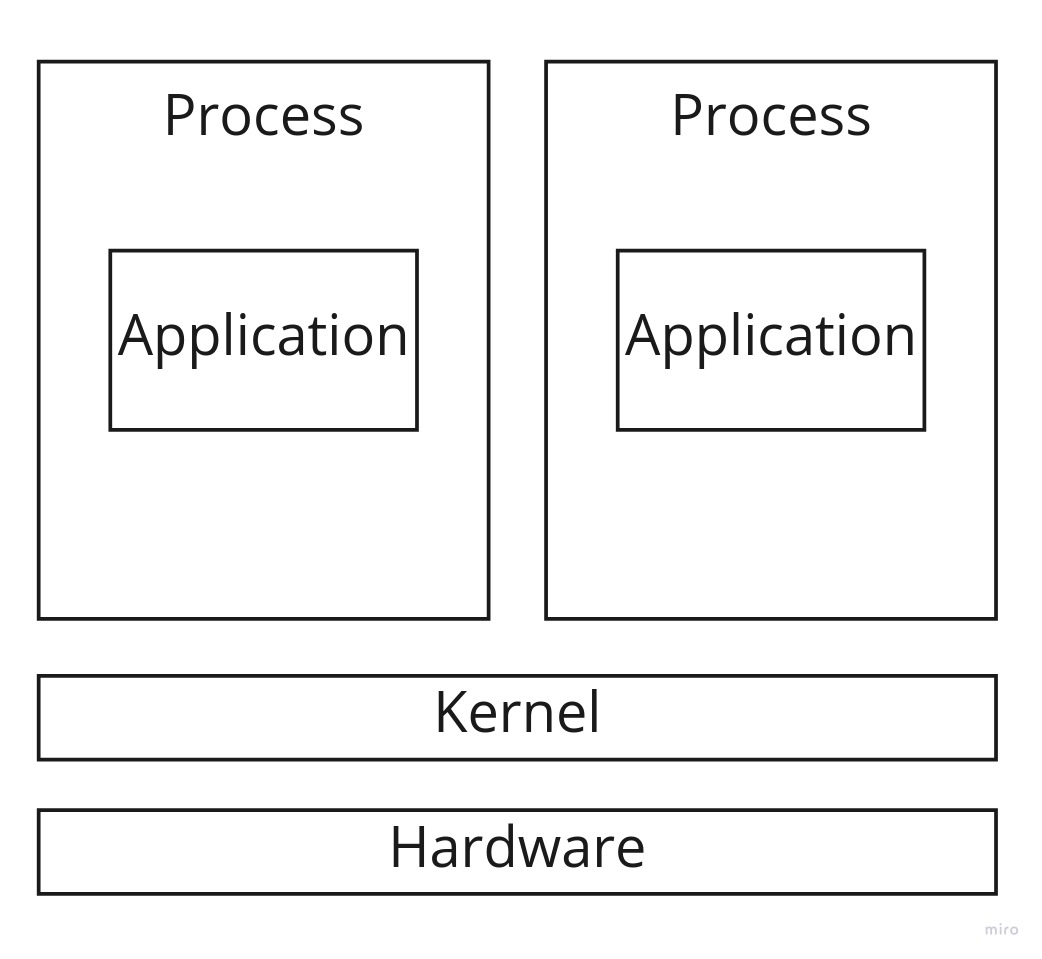
\includegraphics[width=0.6\textwidth]{images/fundamentals/kernel-virt-arch.jpg}
        \caption{Virtualisation using a shared kernel that constantly assures noninterference by 
                handling service requests from user processes. Kernel has full control of the system
                and represents a single point of failure. There are no mechanisms to reestablsh 
                system health.}
        \label{images:fundamentals/kernel-virt-arch.jpg}
    \end{subfigure}%
    \hfill
    \begin{subfigure}[b]{0.45\textwidth}
        \centering
        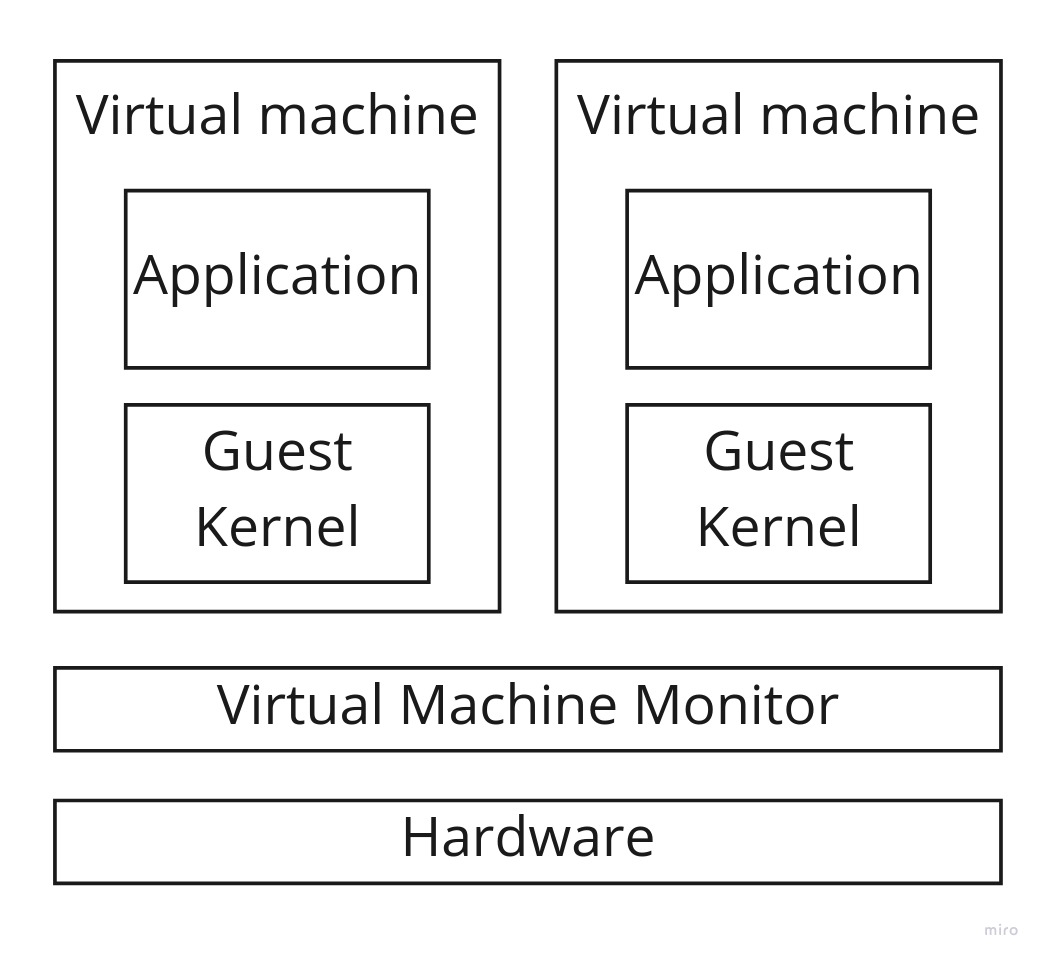
\includegraphics[width=0.6\textwidth]{images/fundamentals/full-virt-arch.jpg}
        \caption{Virtualisation using multiple independent kernels, each ensuring noninterference. 
                If one kernel fails, the virtual machine monitor can reclaim the respective resources or 
                perform operations that reconstruct the virtual machine's state from a health checkpoint.}
        \label{images:fundamentals/full-virt-arch.jpg}
    \end{subfigure}
\caption{Architectural comparison between shared-kernel virtualisation (\ref{images:fundamentals/kernel-virt-arch.jpg})
         and multi-kernel virtualisation using a virtual machine monitor (\ref{images:fundamentals/full-virt-arch.jpg})}
\label{images:fundamentals/virt-arch}
\end{figure}
\subsubsection{Performance}
